\documentclass[12pt, a4paper]{article} 
\usepackage{amsmath,amsfonts,amssymb,amsthm,mathtools}  
\usepackage{fontspec}         % пакет для подгрузки шрифтов
\setmainfont{Roboto}          % задаёт основной шрифт документа
\usepackage{unicode-math}     % пакет для установки математического шрифта
\setmathfont{Asana Math}      % шрифт для математики
\usepackage{polyglossia}      % Пакет, который позволяет подгружать русские буквы
\setdefaultlanguage{russian}  % Основной язык документа
\setotherlanguage{english} 
\begin{document}
\section{Факты обо мне}
\begin{enumerate}
\item Яковлева Ирина Игоревна.
\item Если сложить все цифры из даты рождения, то получится $2^5$.
\item Живу в Москве.
\item Знаю английский и французский,но умудрилась забыть немецкий.
\item Когда-то (совсем недавно) собиралась поступать на геофак,но оказалась на экономе (это слишком долгая история).
\item Пишу НИР по макроэкономике.
\item Люблю эконометрику,макроэкономику.
\item Не совсем дружу с микрой и торами.
\item Всегда пишу $\sigma$ и $\delta$ одинаково.
\item Всегда пишу черной ручкой, только в исключительных случаях-синей.
\end{enumerate}
\section{Фото}
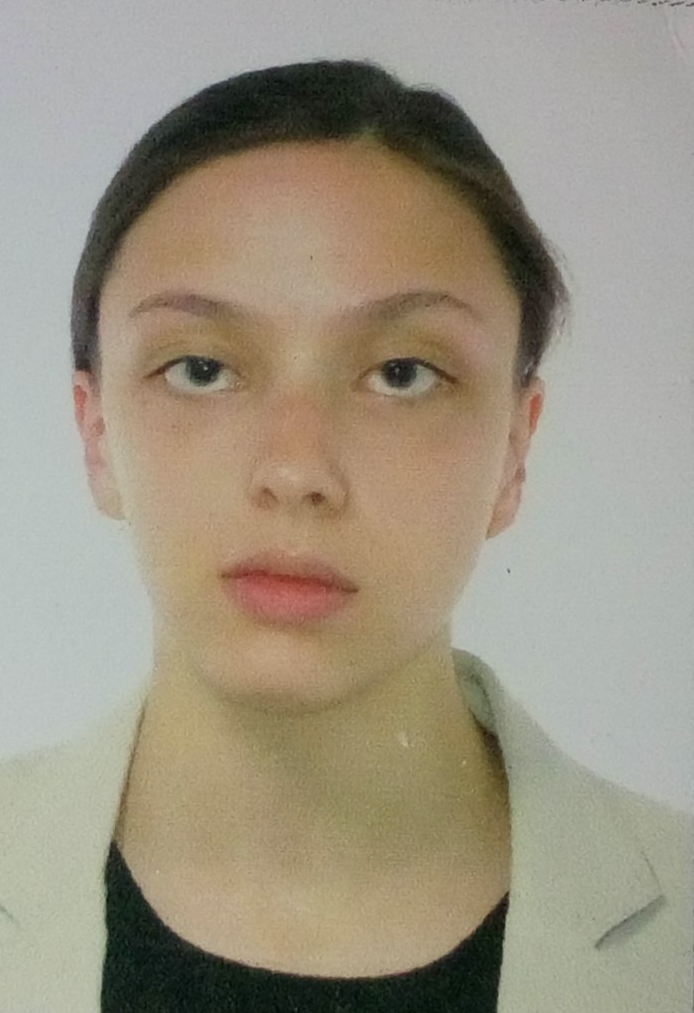
\includegraphics[scale=0.09]{foto.png}
\section{Формулы}
\subsection{Любимые формулы}
\begin{equation}\tag{æ} \label{e1}\lim\limits_{x \to 1} \frac{\sin x}{x}
\end{equation}
\begin{equation}\tag{ææ} \label{e2}\int \frac{dx}{x^2-a^2}=\frac{1}{2a}\left|\frac{x-a}{x+a}\right|+C
\end{equation}
\begin{equation}\tag{æææ}\label{e3} defl=\frac{\sum\nolimits_{k=1}^n p_1 q_1}{\sum\nolimits_{k=1}^n p_0 q_1}
\end{equation}
\begin{equation}\tag{ææææ}\label{e4}\begin{vmatrix} a & b \\ c & d \end{vmatrix}=ad-bc
\end{equation}
\begin{equation}\tag{æææææ}\label{e5}\int\limits_a^{\infty}f(x)dx=\lim\limits_{b \to 1}\int\limits_a^b f(x)dx 
\end{equation}

\subsection{Нелюбимая формула}

\begin{multline*}\tag{ææææææ}\label{e6}
\frac{z_1}{z_2}=\frac{|z_1|}{|z_2|} \cdot \frac{\cos \varphi_1+i\sin \varphi_1}{\cos \varphi_2+\sin \varphi_2} \cdot \frac{\cos \varphi_2-i\sin \varphi_2}{\cos \varphi_2-\sin \varphi_2}= \\ = \frac{|z_1|}{|z_2|} \cdot \frac{(\cos \varphi_1 \cos \varphi_2+\sin \varphi_1\sin \varphi_2)+i(\sin \varphi_1 \cos \varphi_2-\cos \varphi_1 \sin \varphi_2)}{\cos ^2\varphi_2+\sin^2 \varphi_2}
\end{multline*}
В пункте \ref{e1} фрмула замечательного предела,она здорово помогает в решении многих простых и не очень заданий. Следующая формула для вычисления неопределенного интеграла \ref{e2} кажется на первй взгляд громоздкой, но легко запоминается, любой любитель интегралов по должному оценит ее. Далее формула \ref{e3} из макроэкономики и статистики самая простая из всех имеющихся формул, наверное, проще может быть только $Y=C+I+G+Nx$.Формула \ref{e4} мне нравится просто потому, что люблю считать определители и не только 2-ого порядка, а эта как пример.Ну а \ref{e5} помогает немного разобраться с неопределенными интегралами. Эта формула довольно-таки простая, но на перый взгляд может показаться ненавистной из-за обилия $sin$ и $cos$.
\end{document}. 
